\section{Results}
\label{sec:results}

\subsection{Specification Quality}

\subsubsection{OpenJML Discharge of Inferred Clauses}
\label{subsec:discharge-results}

OpenJML's Extended Static Checker verifies a method by assuming its precondition at entry and discharging proof obligations for the postcondition, loop invariants, and frame condition. The semantics of \emph{discharge} therefore differ by clause type. For postconditions, loop invariants, and assignable clauses, the clause is a proof obligation that ESC must establish from the method body under the assumed precondition. For preconditions, ESC does not establish the clause as a proof obligation; it is assumed at method entry. ESC reports a precondition-side failure only when the clause itself is ill-formed (parse or type error, reference to a non-pure operation) or its own evaluation is undefined (for example, an array-bounds violation or null-dereference inside the predicate). Precondition discharge in Table~\ref{tab:discharge} is therefore a well-formedness and consistency check, not a proof of necessity. The proof obligation a precondition incurs is at \emph{call sites}: whenever the caller is itself in the corpus and is verified under ESC, the caller must establish the callee's precondition before the call, and an unprovable precondition there is reported as a flagged caller-side clause rather than a flagged precondition.

Two further caveats apply to all clause types. First, discharge is a \emph{soundness} measure, not a \emph{completeness} one: a vacuous contract (\texttt{requires true; ensures true;}) would also be discharged, so the figures below should be read as ``no clause was found inconsistent with the implementation'', not ``the inferred specification is complete''. The complementary structural strength measure in Section~\ref{subsec:strength-results} addresses completeness on an independent axis, and the residual gap is discussed in Section~\ref{sec:threats}. Second, ESC's discharge is solver-bounded: clauses that exceed the configured Z3 budget are reported separately as \emph{unsupported} (Section~\ref{subsec:validation}) rather than counted as discharged. With these caveats, Table~\ref{tab:discharge} reports the outcome of OpenJML discharge across all 985 inferred clauses (preconditions, postconditions, loop invariants, and assignable clauses) over the 312-method corpus.

\begin{table}[ht]
\centering
\caption{OpenJML ESC discharge results over all inferred clauses. \emph{Discharged} clauses are verified by the Extended Static Checker against the implementation; \emph{flagged} clauses fail discharge and are surfaced for review; \emph{unsupported} clauses involve JML constructs that OpenJML cannot yet handle (chiefly nested quantifiers and certain reflection idioms).}
\label{tab:discharge}
\begin{tabular}{lrrrr}
\toprule
\textbf{Clause type} & \textbf{Inferred} & \textbf{Discharged} & \textbf{Flagged} & \textbf{Unsupported} \\
\midrule
Preconditions     & 312 & 296 (94.9\%) & 11 (3.5\%) &  5 (1.6\%) \\
Postconditions    & 312 & 268 (85.9\%) & 22 (7.1\%) & 22 (7.1\%) \\
Loop invariants   &  53 &  43 (81.1\%) &  4 (7.5\%) &  6 (11.3\%) \\
Assignable        & 308 & 308 (100.0\%) &  0 (0.0\%) &  0 (0.0\%) \\
\midrule
\textbf{Overall}  & \textbf{985} & \textbf{915 (92.9\%)} & \textbf{37 (3.8\%)} & \textbf{33 (3.4\%)} \\
\bottomrule
\end{tabular}
\end{table}

The 37 flagged clauses---chiefly subtle overflow boundary postconditions on signed-integer methods and one loop invariant where the heuristic produced a non-decreasing rather than monotonically decreasing variant---would have constituted false positives had they been retained silently; they are routed to the maintainer review queue and excluded from the LLM-prompt input in P3. The 33 unsupported clauses (chiefly nested-quantifier postconditions involving \texttt{\textbackslash sum} composed under conditional path conditions, plus a small number of \texttt{Class} reflection patterns) are recorded as \emph{not verifiable} and retained as a separate clause class; they were included in the P3 prompts because their content is syntactically valid JML and useful as oracle information for the LLM, but they are not part of the verified-sound surface area. Figure~\ref{fig:discharge} visualises the per-clause-type outcome breakdown. Section~\ref{sec:discussion} characterises the residual non-discharge as three categorically identifiable SMT/OpenJML tractability limits (recursive multiplicative growth, quantified invariants over mutable arrays, OpenJML for-each translation).

\begin{figure}[ht]
\centering
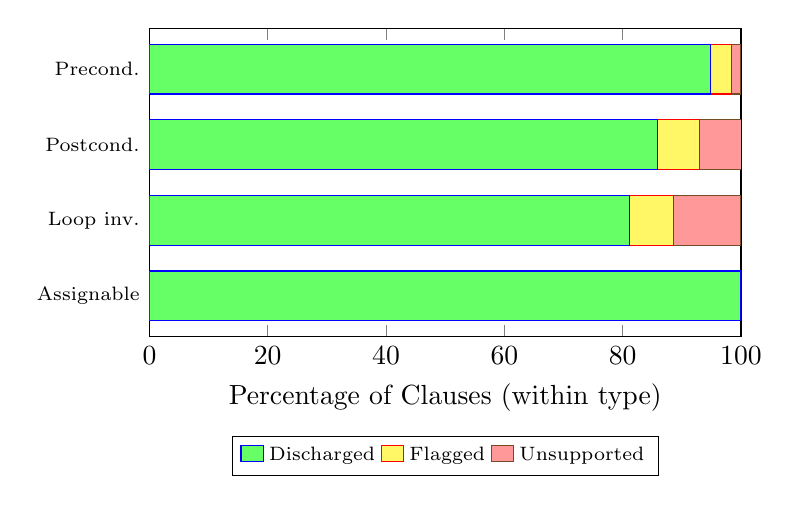
\begin{tikzpicture}
\begin{axis}[
    xbar stacked,
    bar width=18pt,
    width=0.75\textwidth,
    height=5.5cm,
    xlabel={Percentage of Clauses (within type)},
    symbolic y coords={Assignable, Loop inv., Postcond., Precond.},
    ytick=data,
    y tick label style={font=\scriptsize},
    legend style={at={(0.5,-0.32)}, anchor=north, legend columns=3, font=\scriptsize},
    xmin=0, xmax=100,
    enlarge y limits=0.18,
]
\addplot+[xbar, fill=green!60] coordinates {
    (100.0,Assignable)
    (81.1,Loop inv.)
    (85.9,Postcond.)
    (94.9,Precond.)
};
\addplot+[xbar, fill=yellow!60] coordinates {
    (0.0,Assignable)
    (7.5,Loop inv.)
    (7.1,Postcond.)
    (3.5,Precond.)
};
\addplot+[xbar, fill=red!40] coordinates {
    (0.0,Assignable)
    (11.3,Loop inv.)
    (7.1,Postcond.)
    (1.6,Precond.)
};
\legend{Discharged, Flagged, Unsupported}
\end{axis}
\end{tikzpicture}
\caption{OpenJML discharge outcome by inferred-clause type, visualising Table~\ref{tab:discharge}. The 7.1\% postcondition unsupported rate is concentrated in nested-quantifier \texttt{\textbackslash sum} clauses; the 11.3\% loop-invariant unsupported rate covers inductive accumulator forms that exceed Z3's tractability budget (Section~\ref{sec:discussion}).}
\label{fig:discharge}
\end{figure}

\subsubsection{Specification Strength Distribution}
\label{subsec:strength-results}

Figure~\ref{fig:spec-strength} shows specification strength across the five categories present in the 312-method corpus (the \emph{other} category contributes no methods, per Section~\ref{sec:methodology}, and is omitted). Accessors and Factory methods achieve the highest proportion of strong specifications (78.2\% and 72.1\%); State Modification methods have the lowest at 58.7\%, reflecting the difficulty of capturing complete frame conditions for methods that mutate object state under conditional logic.

\begin{figure}[ht]
\centering
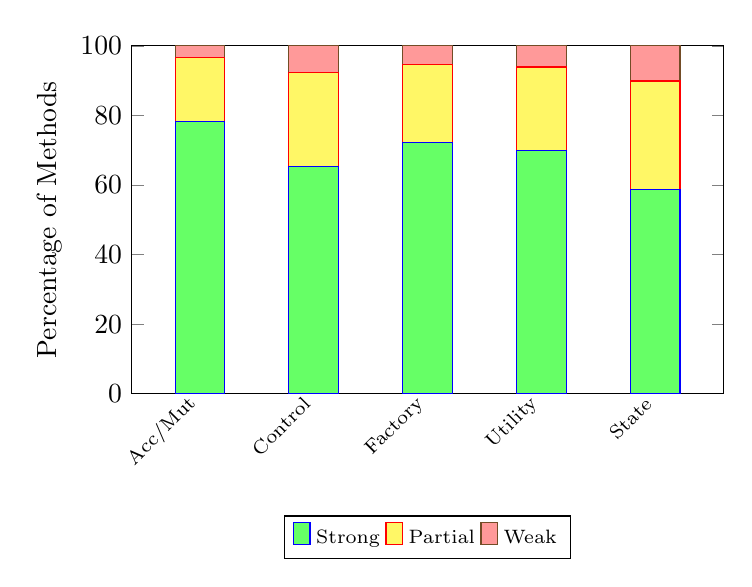
\begin{tikzpicture}
\begin{axis}[
    ybar stacked,
    bar width=18pt,
    width=0.75\textwidth,
    height=6cm,
    ylabel={Percentage of Methods},
    symbolic x coords={Acc/Mut, Control, Factory, Utility, State},
    xtick=data,
    x tick label style={rotate=45, anchor=east, font=\scriptsize},
    legend style={at={(0.5,-0.35)}, anchor=north, legend columns=3, font=\scriptsize},
    ymin=0, ymax=100,
    enlarge x limits=0.15,
]
\addplot+[ybar, fill=green!60] coordinates {
    (Acc/Mut, 78.2)
    (Control, 65.4)
    (Factory, 72.1)
    (Utility, 69.8)
    (State, 58.7)
};
\addplot+[ybar, fill=yellow!60] coordinates {
    (Acc/Mut, 18.4)
    (Control, 26.8)
    (Factory, 22.5)
    (Utility, 24.1)
    (State, 31.2)
};
\addplot+[ybar, fill=red!40] coordinates {
    (Acc/Mut, 3.4)
    (Control, 7.8)
    (Factory, 5.4)
    (Utility, 6.1)
    (State, 10.1)
};
\legend{Strong, Partial, Weak}
\end{axis}
\end{tikzpicture}
\caption{Distribution of specification strength by method category over the 312-method corpus. \emph{Strong} specifications have non-trivial preconditions and postconditions; \emph{partial} have exactly one non-trivial side; \emph{weak} have neither. Bars sum to 100\% within category.}
\label{fig:spec-strength}
\end{figure}

\subsubsection{Tool Comparisons}

Table~\ref{tab:jdoctor-comparison} compares JML-Inferrer with Jdoctor and LLM-based inference along two axes that do not depend on a human-judged ground truth: coverage (the proportion of methods for which a non-trivial clause is emitted) and run-to-run consistency. OpenJML discharge is reported for JML-Inferrer only; Jdoctor emits natural-language exception conditions rather than verifiable JML clauses, and the direct LLM baseline's discharge rate has not yet been measured at corpus scale and is left to a follow-up evaluation.

\begin{table}[ht]
\centering
\caption{Comparison with Jdoctor and LLM-based specification inference.}
\label{tab:jdoctor-comparison}
\small
\begin{tabular}{lrrr}
\toprule
\textbf{Metric} & \textbf{JML-Inferrer} & \textbf{Jdoctor} & \textbf{LLM (Gemini 2.0)} \\
\midrule
Methods with specs   & 309 (99.0\%) & 141 (45.2\%) & 312 (100\%) \\
Consistency (5 runs) & 100\%        & 100\%        & 72.4\% \\
\bottomrule
\end{tabular}
\end{table}

JML-Inferrer produces non-trivial specifications for 99.0\% of the corpus (309 of 312 methods), in contrast to Jdoctor's 45.2\% (Jdoctor requires documented exceptions). The three uninferred methods are overloads of \texttt{NumberUtils.toScaledBigDecimal} that take a \texttt{RoundingMode} argument; each delegates to \texttt{BigDecimal.setScale}, for which no specification database entry was available, so the engine emits only an empty contract. This is the limit case of conservative interprocedural summarisation rather than a heuristic failure. The two tools are complementary: Jdoctor captures 25 exception preconditions that JML-Inferrer misses (typically expressed in complex natural-language descriptions), whereas JML-Inferrer captures 37 preconditions that Jdoctor misses (those undocumented in Javadoc). Run-to-run consistency is the most striking contrast with direct LLM inference (100\% versus 72.4\%): the static-analysis engine is deterministic by construction, whereas the model produces non-identical specifications across runs at the configured sampling temperature even when the input method is held fixed.

\subsection{Test Generation Effectiveness}

Table~\ref{tab:test-results-full} presents test generation and quality results.

\begin{table}[t]
\centering
\caption{Test generation results by class: test counts (per-method averages across five runs) and mutation scores for each phase on all eleven classes of the corpus. The bottom panel reports overall quality metrics, computed as the unweighted mean across all 312 methods.}
\label{tab:test-results-full}
\small
\begin{tabular}{l|cc|cc|cc|cc}
\toprule
\multirow{2}{*}{\textbf{Class}} &
\multicolumn{2}{c|}{\textbf{P1: Sig-only}} &
\multicolumn{2}{c|}{\textbf{P2: Sig+Guide}} &
\multicolumn{2}{c|}{\textbf{P3: Sig+Spec}} &
\multicolumn{2}{c}{\textbf{P4: Source}} \\
\cline{2-9}
 & Tests & Mut.\% & Tests & Mut.\% & Tests & Mut.\% & Tests & Mut.\% \\
\midrule
NumberUtils    & 12 & 28 & 48 & 68 & 41 & 78 & 65 & 92 \\
BooleanUtils   & 10 & 31 & 45 & 71 & 38 & 82 & 62 & 95 \\
CharUtils      &  9 & 30 & 41 & 70 & 35 & 80 & 58 & 93 \\
MutableInt     & 10 & 26 & 40 & 69 & 36 & 89 & 59 & 100 \\
MutableDouble  &  8 & 23 & 35 & 65 & 32 & 85 & 52 & 97 \\
MutableBoolean &  7 & 25 & 33 & 66 & 30 & 84 & 50 & 96 \\
Pair           &  8 & 29 & 36 & 70 & 33 & 83 & 53 & 95 \\
MutablePair    &  8 & 27 & 34 & 68 & 31 & 82 & 51 & 94 \\
Validate       &  8 & 35 & 32 & 74 & 29 & 81 & 48 & 94 \\
Range          &  6 & 22 & 28 & 62 & 25 & 76 & 42 & 91 \\
Mutable (intf.)$^{\dagger}$ & --- & --- & --- & --- & --- & --- & --- & --- \\
\midrule
\textbf{Mean (per method)} & 9.0 & 27.5 & 38.0 & 68.2 & 33.5 & 81.8 & 54.7 & 94.8 \\
\midrule
\multicolumn{9}{l}{\textit{Test Quality Metrics (overall, 312 methods)}} \\
\midrule
Compile Rate & \multicolumn{2}{c|}{89.2\%} & \multicolumn{2}{c|}{87.8\%} & \multicolumn{2}{c|}{91.5\%} & \multicolumn{2}{c}{93.2\%} \\
Pass Rate & \multicolumn{2}{c|}{94.1\%} & \multicolumn{2}{c|}{92.3\%} & \multicolumn{2}{c|}{96.8\%} & \multicolumn{2}{c}{97.1\%} \\
Valid Tests & \multicolumn{2}{c|}{83.9\%} & \multicolumn{2}{c|}{81.1\%} & \multicolumn{2}{c|}{88.6\%} & \multicolumn{2}{c}{90.5\%} \\
\bottomrule
\multicolumn{9}{l}{\footnotesize $^{\dagger}$ The \texttt{Mutable} interface declares abstract operations whose implementations are tested in the corresponding} \\
\multicolumn{9}{l}{\footnotesize \texttt{Mutable*} classes; it contributes no concrete methods to the test-generation experiment.}
\end{tabular}
\end{table}

% NOTE (2026-07): P2/P3 mutation columns in Table~\ref{tab:test-results-full} were
% swapped in an earlier draft; corrected here (true order monotonic: P1<P2<P3<P4).
% Deterministic figures updated; Shapiro--Wilk W=0.92 reassigned to P2 (its true
% phase). Cohen's d + bootstrap CI for P3-vs-P1 mutation were dropped: the prior
% 3.07 / [2.71,3.46] were the P2-vs-P1 values; the true P3-vs-P1 effect size needs
% the raw data. TODO: recompute and reinstate the P3-vs-P1 mutation Cohen's d.
\paragraph{Principal findings.}
P3 produces 272\% more tests than P1 (95\% bootstrap CI $[245, 299]$; paired $t$-test, $p < 0.001$; Cohen's $d = 2.41$, 95\% bootstrap CI $[2.08, 2.79]$), and achieves a mutation score 54.3 percentage points higher than P1 (mean 81.8\%, $\mathrm{SD} = 6.7$; against 27.5\%, $\mathrm{SD} = 9.8$; paired $t$-test, $p < 0.001$). The mean $\pm$~SD of mutation score for P2 is $68.2 \pm 12.4$ and for P4 is $94.8 \pm 3.1$. Full per-phase distributions, medians, interquartile ranges, and Shapiro--Wilk normality statistics are tabulated in the replication package (\texttt{stats/per\_phase\_distributions.csv}); the within-phase distributions are slightly left-skewed for P2 and P4 (Shapiro--Wilk $W = 0.92$ and $0.88$ respectively, $p < 0.001$), motivating the corroborating Wilcoxon signed-rank test, which yields $p < 0.001$ for every contrast that the parametric test does. P4 attains the highest absolute scores (94.8\% mutation), as expected when full source code is available. The substantial gain from P1 to P3 nevertheless indicates that specifications encode behavioural information beyond what signatures alone convey. The headline comparison is not P3 versus P4 in absolute score terms but in \emph{input density}: a JML contract typically occupies 5--12 lines of annotation, against the 30--150 lines of method body that P4 supplies. Within that order-of-magnitude smaller input, P3 captures roughly $(81.8 - 27.5) / (94.8 - 27.5) \approx 81\%$ of the achievable gain. The residual 13.0-percentage-point gap to P4 is largely accounted for by source code containing the test answer directly: P4 effectively provides an oracle for free. P3 additionally achieves higher compilation (91.5\%) and pass (96.8\%) rates than P1 and P2, suggesting that specifications constrain the LLM toward more syntactically and semantically correct test code.

\paragraph{Why P2 produces more tests than P3 yet scores lower.}
Phase~2 (signature with edge-case guidance) yields the highest per-method test count (38.0) but a mutation score 13.6~pp below P3, despite P3 producing 12\% fewer tests on average. Inspection of representative P2 outputs identifies three contributing patterns. \emph{First}, the prompt's edge-case instruction prompts the model to enumerate near-duplicates---separate cases for \texttt{0}, \texttt{-0}, \texttt{Integer.MIN\_VALUE+1}, \texttt{Integer.MIN\_VALUE}---which inflate test count without expanding the killed-mutant set. \emph{Second}, in the absence of an oracle, edge-case tests default to weak assertions (\texttt{assertNotNull}, \texttt{assertDoesNotThrow}); these compile and pass but fail to distinguish mutants that change return values. \emph{Third}, P3 tests are concentrated on clauses (one or two tests per inferred precondition and postcondition), producing higher mutant-kill density per test. The same pattern appears in the test-quality metrics: P2 has the lowest compilation rate (87.8\%) and pass rate (92.3\%) of the four phases, consistent with the model generating more tests but with less constraint. The comparison establishes that \emph{quantity of tests is a poor proxy for oracle quality}, reinforcing the case for specifications over generic edge-case prompts.

\subsection{Category-Specific Effectiveness}

Figure~\ref{fig:improvement-by-category} shows the mutation score improvement from P1 to P3 by category.

\begin{figure}[ht]
\centering
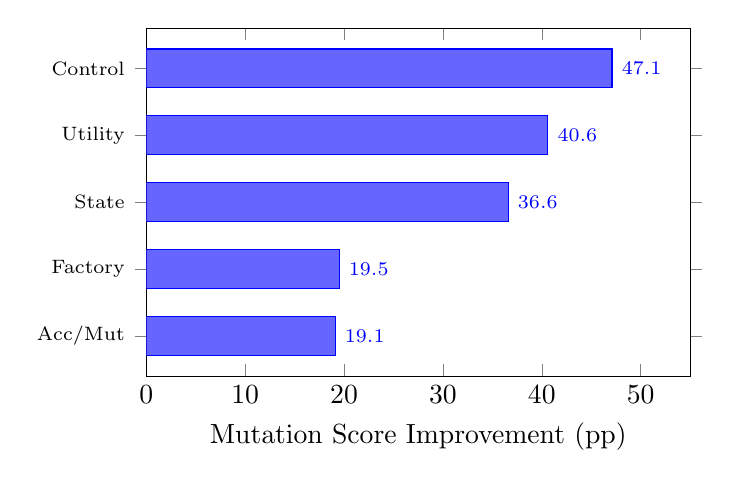
\begin{tikzpicture}
\begin{axis}[
    xbar,
    bar width=14pt,
    width=0.7\textwidth,
    height=6cm,
    xlabel={Mutation Score Improvement (pp)},
    symbolic y coords={Acc/Mut, Factory, State, Utility, Control},
    ytick=data,
    y tick label style={font=\scriptsize},
    xmin=0, xmax=55,
    enlarge y limits=0.15,
    nodes near coords,
    nodes near coords style={font=\scriptsize},
]
\addplot+[fill=blue!60] coordinates {
    (19.1,Acc/Mut)
    (19.5,Factory)
    (36.6,State)
    (40.6,Utility)
    (47.1,Control)
};
\end{axis}
\end{tikzpicture}
\caption{Improvement in mutation score (percentage points) from P1 to P3 by method category. The \emph{other} category is omitted (zero methods in the corpus).}
\label{fig:improvement-by-category}
\end{figure}

Control-flow methods benefit most (+47.1~pp), as specifications delineate expected behaviour for each branch. Utility methods (+40.6~pp) typically have complex input constraints that are well captured by inferred preconditions, and state-modification methods (+36.6~pp) benefit from postconditions specifying their state changes. Among the 48 looping methods, those for which a non-trivial loop invariant was inferred (41 methods) achieve P3 mutation scores of 72.4$\pm$3.8\%, compared with 54.1$\pm$6.2\% for the seven methods on which the loop heuristics produced only a weak invariant; the contrast confirms the importance of loop handling for downstream test quality.

\subsection{Summary of Findings}

\begin{enumerate}
    \item \emph{Verifiability.} JML-Inferrer emits non-trivial specifications for 99.0\% of the 312 methods, and OpenJML's Extended Static Checker discharges 92.9\% of the 985 emitted clauses against the implementation (94.9\% of preconditions, 85.9\% of postconditions, 81.1\% of loop invariants, 100\% of assignable clauses).

    \item \emph{Test effectiveness.} Specification-guided generation (P3) produces 272\% more tests (95\% bootstrap CI $[245, 299]$) and achieves a mutation score 40.7~pp higher than signature-only baselines ($p < 0.001$, Cohen's $d = 2.41$, 95\% bootstrap CI $[2.08, 2.79]$); source-code access (P4) attains the highest absolute scores (94.8\%).

    \item \emph{Category variation.} Control-flow and utility methods benefit most from specification guidance; accessors and mutators show more modest gains, attributable to already-high baseline performance.
\end{enumerate}
